\documentclass{article}

% Language setting
% Replace `english' with e.g. `spanish' to change the document language
\usepackage[english]{babel}
\usepackage[utf8]{inputenc}

% Set page size and margins
% Replace `letterpaper' with `a4paper' for UK/EU standard size
\usepackage[a4paper,top=2cm,bottom=2cm,left=3cm,right=3cm,marginparwidth=1.75cm]{geometry}

% Useful packages
\usepackage{amsmath, amssymb, amsthm}
\usepackage{geometry}
\usepackage{graphicx}
\usepackage{physics} % For nicer derivatives, etc.
\usepackage{enumitem}
\usepackage{hyperref} % For clickable links
\usepackage{xcolor}
\usepackage{fancyhdr} % For header and footer
\usepackage{tikz}

\renewcommand{\qedsymbol}{$\blacksquare$} % Define the end of proof symbol

%--- Theorem, Definition, etc. Environments ---
\theoremstyle{definition}
\newtheorem{definition}{Definition}[section]
\newtheorem{example}{Example}[section]

\theoremstyle{plain}
\newtheorem{theorem}{Theorem}[section]
\newtheorem{lemma}{Lemma}[section]
\newtheorem{proposition}{Proposition}[section]
\newtheorem{corollary}{Corollary}[section]

\theoremstyle{remark}
\newtheorem{remark}{Remark}[section]

% --- Header and Footer ---
\pagestyle{fancy}
\fancyhf{} % Clear header and footer
\renewcommand{\headrulewidth}{0.4pt} % Set header line thickness
\renewcommand{\footrulewidth}{0.4pt} % Set footer line thickness
\fancyhead[C]{\footnotesize Lecture \thesection: Introduction} % Center Header with section
\fancyhead[R]{\footnotesize \today}  % Right Header
\fancyfoot[C]{\footnotesize \thepage} % Center Footer - page number

%--- Color Definitions ---
\definecolor{myblue}{rgb}{0.1, 0.4, 0.7}
\definecolor{mygreen}{rgb}{0.1, 0.7, 0.1}

\hypersetup{colorlinks=true,
            linkcolor=myblue,
            citecolor=mygreen,
            urlcolor=myblue}

\title{Classical Mechanics (McGill University)}
\author{kekeandzeyu}
\date{\today}

\begin{document}

\title{Classical Mechanics (McGill University)}
\author{kekeandzeyu}
\date{\today}

\maketitle

\section{Lecture 2: Lagrangian Mechanics, Euler-Lagrange Equation \& Hamiltonians}

\subsection{Lagrangian Mechanics}

Consider the following simplification: consider the case where the force $\mathbf{F}_\alpha$ is conservative. A force $\mathbf{F}_\alpha$ is \textbf{conservative} if:

\[
    \oint \mathbf{F}_\alpha \, d\mathbf{r}_\alpha = 0
\]

i.e., the work done to change the state of the system is independent of the path through the space of $\mathbf{r}_\alpha$. For a conservative force, 

\begin{align*}
    \mathbf{F}_\alpha &= \mathbf{\nabla}_\alpha V(\mathbf{r}_1,\ ...,\ \mathbf{r}_\alpha) \\
    &= - \frac{\partial}{\partial \mathbf{r}_\alpha} V(\mathbf{r}_1,\ ...,\ \mathbf{r}_\alpha)
\end{align*}

And the work done to change the state of the system from $\mathbf{r}_\alpha$ to $\mathbf{r}_\alpha^\prime$ is $V(\mathbf{r}_\alpha^\prime)-V(\mathbf{r}_\alpha)$. In this class, we will mostly consider conservative forces.

Since $\mathbf{r}_\alpha=\mathbf{r}_\alpha(q_i, t)$, we can write $V(\mathbf{r}_\alpha)$ as:

\[
    V(\mathbf{r}_\alpha)=V(q_i, t)
\]

From \textbf{Chain Rule}, we can get:

\[
    \frac{\partial V}{\partial q_i}=\sum_\alpha \frac{\partial V}{\partial \mathbf{r}_\alpha} \frac{\partial \mathbf{r}_\alpha}{\partial q_i}=-\sum_\alpha \mathbf{F}_\alpha \frac{\partial \mathbf{r}_\alpha}{\partial q_i}=-\mathbf{F}_i
\]

Then for a conservative force, we can get:

\[
    \frac{d}{dt} (\frac{\partial T}{\partial \dot{q}_i}) - \frac{\partial T}{\partial q_i} = -\frac{\partial V}{\partial q_i}
\]

Since $V$ is not a function of $q_i$, we can get:

\[
    \frac{\partial V}{\partial \dot{q}_i}=0
\]

So we can rewrite the EOM above by defining \textbf{Lagrangian} $L=T-V$, $L=L(q_i, \dot{q}_i, t)$

\[
    \frac{d}{dt} (\frac{\partial L}{\partial \dot{q}_i}) - \frac{\partial L}{\partial q_i} = 0
\]

This EOM is called \textbf{Euler-Lagrange Equation}. We can see that for a general dynamic system, if we can compute $L=T-V$, then we can find the equations of motion!

This is a set of $N$ differential equations, one for each DOF, where $N$ is the total number of DOF. Typically, these are $2^{\text{nd}}$ order ODEs for $q_i$.

To summarize, given a system of M parts and N degrees of freedom, it is advised to follow the following steps:

\begin{enumerate}
    \item Identify some dynamic variables $q_i$, and write down $\mathbf{r}_\alpha=\mathbf{r}_\alpha(q_i, t)$, where $\alpha=1,2,...,M$, $i=1,2,...,N$.
    \item Compute $T=\sum_\alpha \frac{1}{2} m_\alpha \dot{\mathbf{r}}_\alpha \cdot \dot{\mathbf{r}}_\alpha$ as a function of $q_i$.
    \item Compute $V=V(\mathbf{r}_\alpha)=V(q_i, t)$.
    \item Let $L=T-V$.
    \item We can get equations of motion: $\frac{d}{dt} (\frac{\partial L}{\partial \dot{q}_i}) - \frac{\partial L}{\partial q_i} = 0$.
\end{enumerate}

\begin{figure}[h]
  \centering
  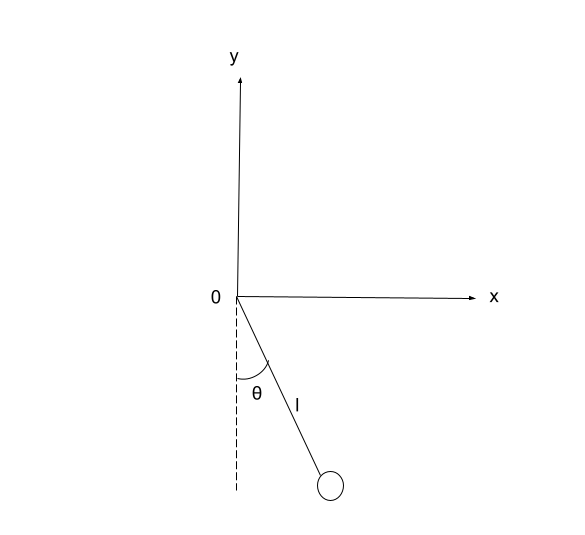
\includegraphics[width=0.8\textwidth]{images/2-1-1.png}
  \caption{Pendulum Example}
  \label{fig:2-1-1}
\end{figure}

For example, let's take a look at the pendulum in Figure \ref{fig:2-1-1}.

\begin{align*}
    x &= l \sin{\theta} \\
    y &= -l \cos{\theta} \\
\end{align*}

So we can get:

\begin{align*}
    \dot{x} &= l \cos{\theta} \cdot \dot{\theta} \\
    \dot{y} &= l \sin{\theta} \cdot \dot{\theta} \\
\end{align*}

So the kinetic energy can expressed as:

\[
    T=\frac{1}{2} m \left(\dot{x}^2+\dot{y}^2\right) = \frac{1}{2} ml^2\dot{\theta}^2
\]

The potential energy is:

\[
    V=-mgy=-mgl\cos{\theta}
\]

\[
    L=\frac{1}{2}ml^2\dot{\theta}^2+mgl\cos{\theta}
\]

From \textbf{Euler-Lagrange Equation} we can get:

\[
    ml^2\Ddot{\theta}+mgl\sin{\theta}=0
\]

\end{document}





